\chapter{Using the Drill Operator}
\label{chapter:UsingTheDrillOperator}

The drill operator presented in chapter \ref{chapter:DrillOperator} provides a unique and novel method for representing the shape of a terrain surface. This chapter explores the operator's utility 
by presenting various enhancements, applications, and uses for the drill operator with regard to accurately and compactly representing terrain data.
% by presenting accuracy tests that show how closely the operator representation can mimic terrain data. These initial accuracy tests are followed by an in depth exploration of various expanded uses and applications of the drill operator.


\section{Initial Accuracy Trials}
\label{section:DrillAccuracyTests}

To determine the feasibility of representing terrain as drills, initial accuracy tests were performed to determine how closely the drill representation modeled the $400 \times 400$ mountainous dataset seen in Figure \ref{figure:mtn2_original}. All tests were performed in Ubuntu 11.04 with a quad-core AMD Phenom II X4 945 Processor, with 8GB of RAM. The code was written in MATLAB.

\subsection{Experimental Methodology}

The three parameters of the system, as described in Chapter \ref{chapter:DrillOperator}, are the threshold used to extract the original terrain's channel network $\tau$, the size of the cross section $w$, and the influence of a drill (size of the representative matrix) $k$. Each of 3 thresholds, 3 cross-section sizes, and 6 influence values were used to build regenerated terrains in the factorial experiment described in this section. 

For each set of parameter values, the total error between the generated terrain and the initial terrain was calculated using a measure for dissimilarity between the two sets.
These metrics take as input two channel networks
($N^{i}_{\tau}$ and $N^{j}_{\tau}$) and return the distance between
them.
 The two metrics used were the standard root mean squares error (RMSE) metric, and the averaged Hausdorff distance (AHD) metric as described in Section \ref{section:DescriptionOfMetrics}.
% by Stuetzle et al. \cite{stuetzle-TerrainDistances}, inspired by the shape analysis techniques discussed in Section \ref{section:ShapeAnalysisTechniques}.

It is important to note that AHD is limited to the channel networks of the terrain, whereas RMSE is applied globally. Limiting RMSE to only $N_{\tau}$ would not give an accurate picture of how close the terrains' hydrography networks are, since the network pixels are found by looking at the global flow pattern. Even if the elevations of the pixels in $N_{\tau}$ are comparable, it does not indicate that the overall terrain shape is similar. In addition, slight variations in the location of the pixels in $N_{\tau}$ would render RMSE unusable. Therefore, the results for both metrics are analyzed in context of their maximum error and what they mean from a physical standpoint.

\subsection{Results and Discussion of Initial Accuracy Trials}
\label{section:DrillAccuracyResultsAndDiscussion}

\begin{figure}
\begin{center}
  \begin{minipage}{0.49\linewidth}
     \includegraphics[height=0.25\textheight,width=0.99\linewidth]{images/RMSE_Graph_CS5.jpg} 

     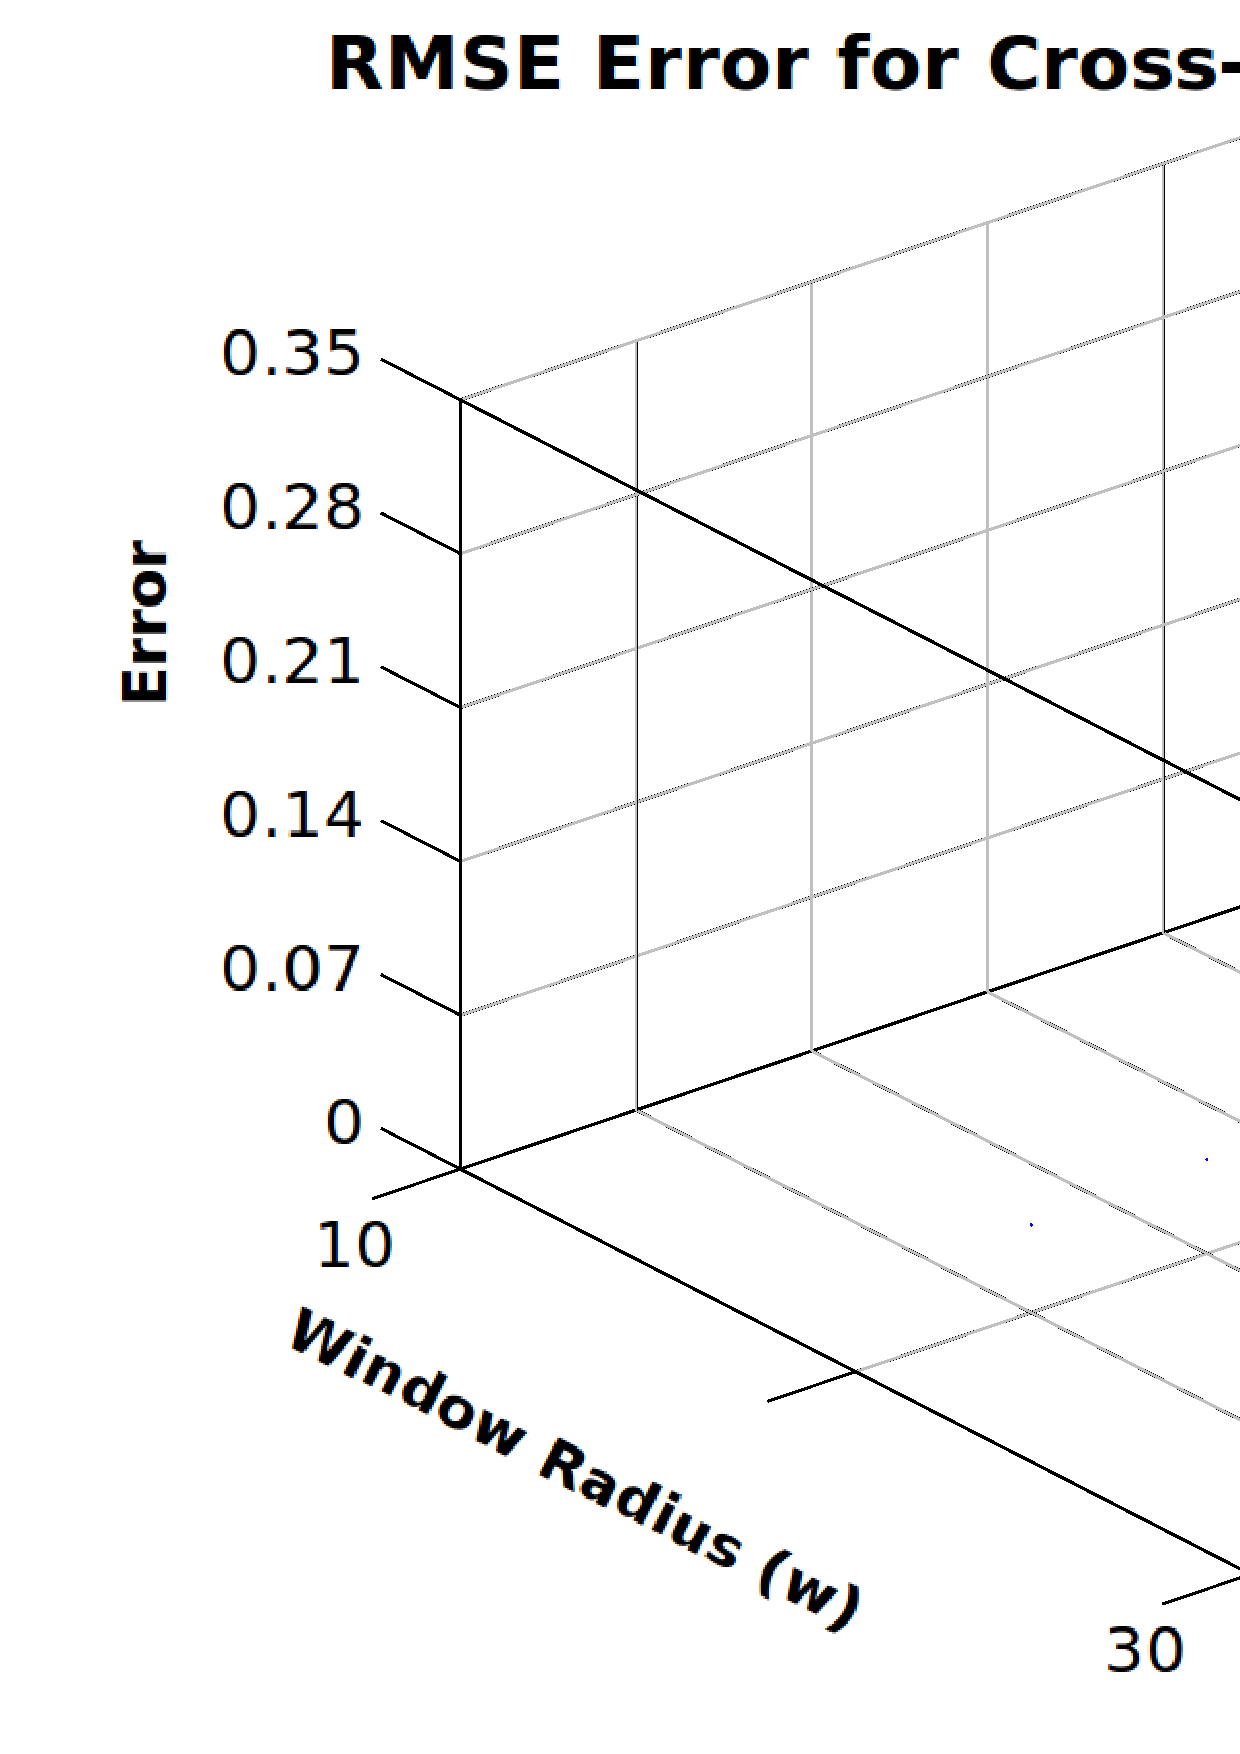
\includegraphics[height=0.25\textheight,width=0.99\linewidth]{images/RMSE_Graph_CS10.jpg}

     \includegraphics[height=0.25\textheight,width=0.99\linewidth]{images/RMSE_Graph_CS15.jpg}  
  \end{minipage}
  \begin{minipage} {0.49\linewidth} 
    \includegraphics[height=0.25\textheight,width=0.99\linewidth]{images/AHD_Graph_CS5.jpg} 
 
    \includegraphics[height=0.25\textheight,width=0.99\linewidth]{images/AHD_Graph_CS10.jpg}

    \includegraphics[height=0.25\textheight,width=0.99\linewidth]{images/AHD_Graph_CS15.jpg}
  \end{minipage}
\end{center}
\caption[The results for the concept tests for the drill operator]{\label{figure:results} The results of accuracy testing. The left column depicts the error measured using the RMSE metric, and the right column depicts error measured used the AHD metric. Each row shows a different value for the cross section window size (parameter $w$). Each metric's data is normalized. Red indicates high error, whereas blue indicates low error, local to each dataset.   }
\end{figure}


\begin{figure}[t]
\begin{center}
  \begin{minipage}{0.49\linewidth} \includegraphics[width=0.99\linewidth]{images/W10_I20_T25.jpg} \\ \centering $\tau=25$, $w=10$, $k=20$ \end{minipage}
  \begin{minipage}{0.49\linewidth} \includegraphics[width=0.99\linewidth]{images/W5_I10_T25.jpg} \\ \centering $\tau=25$, $w=5$, $k=10$ \end{minipage}
\end{center}
\caption[Regenerated terrains with lowest errors]{\label{figure:lowest_errors} The left image depicts the regenerated terrain with the lowest RMSE value, and the right image depicts the regenerated terrain with the lowest AHD error. The parameters responsible for the terrain are listed below the images. }
\end{figure}


The results for the accuracy tests are provided in Figure \ref{figure:results}. The left column of Figure \ref{figure:results} presents the data for the RMSE metric, and the data for the AHD is on the right. The error divisor for RMSE was the total elevation range of the original terrain, whereas the error divisor of AHD was the distance between pixel 0,0 and pixel $n$,$n$, the corners of the terrain. Since elevation is ignored for this divisor, it is possible for AHD error be greater than 1.0. 

$\tau$ values of 25 created considerably denser channel networks than $\tau$ values above 100, and so they are both more accurate and take considerably longer to calculate. The two channel networks can be seen in Figure \ref{figure:mtn2_original}. For reference, the maximum flow value for a pixel in the dataset is 102,245, and a threshold of 25 resulted in a channel network with $\approx19,000$ pixels, whereas a threshold of 100 resulted in a network of $\approx12,000$ pixels. Calculating the drill representation of a terrain with a flow threshold of 25 took approximately three minutes, and times decreased linearly with the increase in threshold value. The time for regenerating the terrain from the drill representation was quicker by approximately a factor of ten. It is important to note that optimization was not a focus at this time, and there exist many techniques that will be utilized in the future to reduce the time the algorithm takes.

There are several observations to be made regarding the accuracy data. The first is that, with ``good'' parameters (meaning none that create outliers in the error data), the accuracy is actually quite high with regard to both RMSE and AHD metrics, between 0.015 and 0.025. As with any algorithm, there is a trade-off between time and accuracy. The lower the threshold, the more pixels in the hydrography network, and so the slower the process, but the more accurate the results become. This is true in every case, and it makes intuitive sense. 

$\tau$ is the most influential parameter with regard to both metrics. 
This makes sense, since the drill is centered around the pixels of $N^{i}_{\tau}$. 
% shape calculation is constrained to pass through the center of $N^{i}_{\tau}$. 
Because AHD measures how close the channel networks are to one another, the more pixels there are in the channels the more likely it is that the channel networks overlap. By nature of the AHD, this will result in very low error. If the channel network is not dense enough, then the drill may not reach much of the terrain at all, and so the RMSE is also very much influenced by the value of $\tau$. More interesting is that the minimum RMSE occurred for when $w = 10$ and $k = 20$. It makes sense that a drill will need some influence over the area around the channel in order to reduce the RMSE, because without it there would be large areas of the terrain untouched by any drill, adding considerably to the overall error (that AHD would ignore). 

From a purely visual standpoint, many of the terrains pass the eyeball test. A side-by-side comparison of the terrains that represent the lowest error for each of the metrics is found in Figure \ref{figure:lowest_errors}. Notice is that the channels do seem to be somewhat wider in the RMSE winner, whereas they are more pointed, but areas of the terrain are missed by drills completely, in the AHD winner. Interestingly, the left image in Figure \ref{figure:lowest_errors} is one of the terrains we deem to be the most ``visually pleasing''. These often have higher $k$ and $w$ values, which may be a result of drills that flatten artifacts out of the terrain. This result demonstrates why, when choosing parameters for the drill operator, it is often smart to take both error metrics into account.


\section{Families of Functions for Drill Shape}
\label{section:FamiliesOfFunctions}

\begin{figure}[t]
  \caption[Graphical representations of drill shape functions.]{\label{figure:FamiliesOfFunctions} This figure shows graphical 2D examples of each of the families of functions making up several possible drill shapes.}
\end{figure}

\fbox{I will make a figure of the function families tested}


\begin{table}[t]
  \centering
  \begin{tabular}{ | c | c | c | c | }
    \hline
      & \textbf{AHD} & \textbf{RMSE} & \textbf{SSRMSE} \\
    \hline
    \textbf{Linear}&&&  \\
    \hline
    HILL1 & 0.0572 & 0.0700 & 0.1013 \\
    HILL2 & 0.1848 & 0.1564 & 0.0923 \\
    HILL3 & 0.0563 & 0.0394 & 0.0644 \\
    MTN1 & 0.0483 & 0.0517 & 0.1000 \\
    MTN2 & 0.0285 & 0.0141 & 0.0819 \\
    MTN3 & 0.0383 & 0.0379 & 0.0764 \\
    \hline
    \textbf{Quadratic}&&& \\
    \hline
    HILL1 & 0.0673 & 0.1230 & 0.1581 \\
    HILL2 & 0.1840 & 0.1581 & 0.1022 \\
    HILL3 & 0.0678 & 0.0965 & 0.1888 \\
    MTN1 & 0.0568 & 0.1364 & 0.2403 \\
    MTN2 & 0.0192 & 0.0184 & 0.1080 \\
    MTN3 & 0.0362 & 0.0771 & 0.1477 \\
    \hline
    \textbf{Cubic}&&&  \\
    \hline
    HILL1 & 0.2757 & 0.3413 & 0.3803 \\
    HILL2 & 0.1820 & 0.1674 & 0.0894 \\
    HILL3 & 0.2060 & 0.2412 & 0.3155 \\
    MTN1 & 0.6620 & 0.5032 & 0.1197 \\
    MTN2 & 0.0160 & 0.2521 & 0.1227 \\
    MTN3 & 0.5117 & 0.4783 & 0.1041 \\
    \hline
  \end{tabular}
  \caption[Minimum error values in tests for different drill shape function families.]{\label{table:FamiliesOfFunctionsResults} This table presents the minimum error found for each of RMSE, AHD, and SSRMSE metrics, divided by function family. The top third of the table refers to data for linear drill shapes, the middle third to quadratic drill shapes, and the bottom third to cubic drill shapes. The results for each of the six datasets found in Figure \ref{figure:SixDatasets} is reported.}
\end{table}

% Properly determining the drill shape can have a profound effect on the accuracy and flexibility of the operator. 
This section explores various drill shapes that can be used to represent the terrain surface.
The drill shape can be represented by any two-dimensional curve (not necessarily by a single-valued function). 
As a preliminary investigation into the effect of the drill shape, the following polynomial curves were investigated:
% This work investigates polynomial and logistic functions. 

\begin{itemize}
  \item Linear functions: Polynomials of degree one
  \item Quadratic functions: Polynomials of degree two
  \item Cubic functions: Polynomials of degree three
  \item Logistic functions
\end{itemize}

\fbox{FIX THE GRAPHIC}

\noindent Graphical examples of each of these families of functions can be seen in Figure \ref{figure:FamiliesOfFunctions}. Each family allows for arbitrarily steep slope (although slight modifications are required for vertical and negative slopes, though those can be incorporated with slight modifications to the fitting functions). 

A test was performed comparing the accuracy of each drill shape. Each test was a factorial experiment using the same three parameters described in Section \ref{section:DrillAccuracyTests} (channel network threshold, drill influence, cross-section size). For these experiments, the threshold was determined by the percentage of pixels to be extracted, and so $r$ was used as the third parameter in lieu of $\tau$. Using a percentage to define the extraction threshold provides a better idea of how much of the terrain is included in the channel network, and, more importantly, how many pixels are required to encode the terrain.

Three of the error metrics defined in Section \ref{section:DescriptionOfMetrics} were used for this test: AHD, RMSE, and SSRMSE. Beyond the fact that slope is an important terrain characteristic, the SSRMSE metric was included with AHD and RMSE (used in the test in Section \ref{section:DrillAccuracyTests}) in these tests because visual inspection of the results from Section \ref{section:DrillAccuracyResultsAndDiscussion} revealed that the peak areas between channels were pointed more than the original terrain. The slope-based metric will penalize this behavior more than RMSE.

Each possible drill function was tested in a factorial experiment. For each segment of the channel network, a single drill shape was determined (minimizing the number of fittings needed). Values up to 30 were tested for $r$ and $w$, and in the interest of limited time $k$ was set to the value of $w$. Logistic functions were immediately thrown away, as their results were incredibly bad. However, the results for the other three function families are presented in Table \ref{table:FamiliesOfFunctionsResults}.

Each of the values in the table is the minimum error found for each respective metric and dataset. Once again, the density of the pixels in the channel network is the most important parameter. In general, as the value of $r$ increases (with the number of drill operators), the accuracy of the representation increases as well. This is not always the case, but in most instances it is true. This means that $r$ can act as a tuning parameter for compression schemes, since it (more than the other parameters) controls the accuracy of the representation.

Somewhat surprisingly, the best results are almost universally within the linear group. A linear drill shape represented each terrain dataset within (approximately) 10\% error in each metric, with the exception of HILL2. The linear drill provided particularly good results for the more mountainous data in all three metric categories, and both HILL1 and HILL3 are adequately represented.

A closer inspection of HILL2 reveals that the dataset is very plateaued, and has few if any clearly defined channels. It is safe to say that, while the drill representation is capable of modeling hilly and plateaued terrains, it is better suited for more mountainous data, especially those with clearly defined channels. This may be due to the nature of the drill shape, or it might be due to the nature of the terrain. 
% method used to extract the channel network. 
On a flat or plateaued terrain, there are many instances in which determining neighbor flow requires tie-breaking procedures (as discussed in Section \ref{section:ChannelNetworkExtraction}). Major network extraction methods handle this differently, and so it is possible that, given a terrain with many ties among neighbors, two methods might produce radically different (and somewhat unstructured) networks. 
Extracted flow direction fields are not always intuitive and obvious on flatter terrain.

The results become increasingly worse as the degree of the polynomial family also increases. The cubic family is, for the most part, not a suitable representation of the surface. The quadratic family provides good-to-poor results, depending on the dataset. Once again, HILL2 is not modeled effectively, and MTN1 and HILL1 have poor RMSE results but good AHD results. This implies that the quadratic drills accurately model (and maintain) the channel networks, but fail to accurately model the data outside of them. 

Overall, the linear drill shape is adequate for modeling various terrain surfaces. The less detailed the surface, and the less clear the channel network to be extracted, the greater the chance for random outliers in error (such as HILL2). This suggests a procedure for trying multiple drill shapes for each channel individually, which is discussed in Section \ref{section:FutureWork}.

% \section{Interpolating Drill Shapes}

In addition to testing these three drill shape families, the same test was run again using a procedure that assigned a single drill to an entire channel segment, rather than a single pixel. The drill shape was calculated at the first and last pixel of each segment, and for the pixels in between its shape was dynamically altered using linear interpolation. The results of this similar test were very close to the results listed in Table \ref{table:FamiliesOfFunctionsResults}, with 10\% for most data points and with no outliers. 

Because linear drill shape is the most accurate, and because it is equally as effective to assign a single dynamic drill shape to an entire channel, it is possible to store several pixels' worth of surface data very compactly by storing a single value for the start pixel, Freeman Chain Codes for the length of the channel, and two values for the drill shape polynomial. Therefore, a terrain can be effectively compressed. 

Finally, and perhaps most importantly, when a drill is assigned to and interpolated through a channel, and this process is consistent for all channels in the network, then local minima cannot appear in the regenerated terrain. This assumes that each segment travels downhill. Because the drill shape is monotonically increasing, the minimum of the terrain in any given local area must be the center of some drill, which is guaranteed to be at a higher elevation (lower priority) than its downstream neighbor in the channel network. This is true for all pixels all the way to the sink of the network, and therefore local minima cannot exist, satisfying one of the criteria of legal terrain generation.

\section{Compression Using the Drill Operator}
\label{section:TerrainCompression}

One of the natural applications of the drill representation is terrain compression. 
As discussed in Section \ref{section:TerrainDataCompression}, terrain data is often compressed with image compression techniques. These techniques achieve very good compression ratios and include progressive transmission which allows the user to provide either a data loss or a compression ratio threshold for near-lossless compression techniques.

However, these techniques ignore important terrain characteristics. For instance, the JPEG algorithm tends to blur sharp edges in images, thus inadvertently smoothing the image surface. The goal of this work is to preserve the important characteristics of the surface, specifically its hydrographical information. The drill representation seems a natural choice for this type of compression, since it is restricted to the pixels of the drainage network and mimics the physics of terrain generation. Therefore, this section presents a method for near-lossless terrain compression using the drill representation.

There are several considerations and sub-problems to tackle when determining how to store terrain data as compactly as possible. The first is to limit the encoding of a single drill. The second is to compress the locations of the drill, i.e. how to compress the drainage network. The final consideration is whether it is possible to allow for the user to determine a compression threshold, either with regard to storage or accuracy.

\subsection{The Compression Scheme}
\label{section:CompressionScheme}

\begin{figure}[t]
  \centering
  \includegraphics[width=0.6\textwidth]{images/LineGeneralization_cropped.png}
  \caption[A simple example of line generalization.]{\label{figure:LineGeneralization}A simple example of line generalization, where a curve (blue) is represented by a working segment represented by 4 points along the curve connected by three line segments (red). Adding more points increases the accuracy of the generalization.}
\end{figure}


The steps to compressing the a terrain as a drill representation are as follows:

\begin{enumerate}
  \item Compress each segment of the drainage network using Freeman Chain Coding or line generalization.
  \item Encode each drill as an initial pixel and a drill shape.
  \item Compress the drill encoding.
  \item (Optional) Apply further compression techniques, such as 7Zip.
\end{enumerate}

As discussed in Section \ref{section:FamiliesOfFunctions}, a single drill can be encoded per segment of the channel network without significant loss of accuracy. In lieu of this, the various segments of the drainage network can be compressed using a scheme such as Freeman Chain Coding \cite{Freeman:1974:CPL:356625.356627} or line generalization \cite{Ramar72:Polygonalapproximation}. 

Freeman Chain Coding is a lossless method of compressing a line segment in an 8-directional system by storing the initial pixel location and then a chain of movement directions. The simplicity of the representation allows for additional compression, since each subsequent direction can be stored in 3 bits. In addition, taking advantage of the tendency for flows to travel in the same direction for long distances allows each segment to be compressed further by simple run length encoding, or more complex lossless compression.
 
Alternatively, line generalization is a lossy method of compressing a line segment by creating a current guess for the line, called the \textit{working segment}, initialized with the first and last pixel of the line.
% starting with the beginning and ending pixel of a segment and drawing a line between them. 
% This is the initial guess for the line segment. 
The furthest pixel from the working segment, using the 2-norm distance in pixel space, is then added to it, and a new guess is created with all the pixels in the working segment. This process is repeated until the desired accuracy or compression ratio is achieved. An example of this process can be seen in Figure \ref{figure:LineGeneralization}.

Since each line segment of the drainage network is now indexed in the encoding by its starting pixel, each drill can be stored in order of the index of the corresponding segment, and so only needs to be encoded as the shape. The drill encoding then becomes a $2 \times n$ matrix, where $n$ is the number of drills, and can be compressed with any lossless matrix compression scheme that is convenient. 

What is important to note is that Freeman Chain Coding is lossless, so if it is used along with a lossless compression of the drill matrix, the only accuracy lost by this scheme is found in the actual representation itself. To a degree, this is unnecessary since most terrain data is inherently inaccurate to begin with. However, by making the accuracy of the compression (either using lossless, or bounded with line generalization) adjustable, there is an additional level of control put in the hands of the user.

Once the compressed files are written, then can be compressed further with file archive problems such as 7Zip \cite{7z-Pavlov} and gzip. Both provide additional compression with minimal data loss.

\subsection{Results and Discussion of Compression Testing}

The six datasets shown in Figure \ref{figure:SixDatasets} were compressed using the scheme presented in Section \ref{section:CompressionScheme}, as well as image compression techniques PNG and JPEG, and archiving technique 7Zip.
For these tests, the drill was compressed by converting the ASCII data into binary data and storing the Freeman Chain Codes as an optimal series of 3-bit sequences.
The PNG and JPEG files were created using the respective MATLAB implementations, and the 7Zip files were created using the default Ubuntu 11.04 compression option. For the JPEG compression, the chosen bit-depth was 12 bits (because 8 was not enough to store the full range of elevations in the data).

The results of these compressions are presented in Table \ref{table:CompressionResults}.

\begin{table}[t]
  \centering
  \begin{tabular}{ | c | c | c | c | c | c |}
    \hline
      & \textbf{Original File Size} & \textbf{Drill Representation} & \textbf{7Zip} & \textbf{JPEG} & \textbf{PNG} \\
    \hline
    HILL1 & 781.3 	& 83.7	& 70.4	& 13.7	& 89.0	\\
    HILL2 & 781.3 	& 161.8 & 101.6	& 20.8	& 138.6	\\
    HILL3 & 781.3 	& 44.8	& 48.7	& 9.3	& 57.7	\\
    MTN1 & 625.4 	& 230.4	& 115.7	& 39.9	& 182.4	\\
    MTN2 & 651.1 	& 8.4	& 130.5	& 36.0	& 145.7	\\
    MTN3 & 625.3 	& 148.5	& 116.0	& 39.9	& 158.6	\\
    \hline
  \end{tabular}
  \caption[Results for compression scheme tests.]{\label{table:CompressionResults} The resulting files sizes (in KB) of files generated using the Drill, 7Zip, JPEG, and PNG compression schemes for each of the six datasets in Figure \ref{figure:SixDatasets}. Each file's original size is given, as well.}
\end{table}

The drill representation used for each dataset was chosen to be the smallest set of operators whose RMSE was below 5\%. The RMSE of each of the other representations was each 0\% (7Zip and PNG, which are lossless) or near 0\% (JPEG). For the drill representation, an additional compression step was applied, using the archive format 7Zip. The additional compression it provided was small, usually only one or two KBs.

The JPEG compression algorithm is very good. With minimal data loss (on a pixel-by-pixel elevation basis), JPEG outperformed all other compression schemes with regard to compression ratio. However, allowing for a 5\% RMSE, the drill compression is able to significantly outperform JPEG and all other schemes on the MTN2 dataset. As presented in Section \ref{section:FamiliesOfFunctions}, the drill is able to very tightly fit the MTN2 dataset, even with very few pixels included in the channel network. This allows for a very small representation to be compressed. 
If the set of operators that provided the smallest error is used, the MTN2 file size grows to \fbox{CHECK THIS FIGURE} 40.0 KB. This is still comparable to the JPEG scheme, and stores more information than JPEG while introducing very little error. 

The PNG scheme performs well for well-structured data with lots of flat areas (HILL1 and HILL3), due to the run-length nature of the scheme. 7Zip performs well for similar reasons, which is why it does not greatly benefit the drill scheme to use it as an additional step since the originally compressed file is very densely packed. 

Like many compression schemes, the drill is dependent upon the structure of the underlying data, most notably the extracted channel network. Improvements in the generalization of the channel network will improve compression ratios while continuing to limit error. As the results for MTN2 prove, it is possible for the drill to accurately and compactly represent a terrain dataset, and the compression scheme introduced in Section \ref{section:TerrainCompression} is feasible. 
% However, improvements to the drill fitting need to be made, whether they be better functions or a generalization of the extracted channel network, before the compression can be widely used for many datasets.
To make the scheme a practical reality, further development of drill fitting techniques is necessary, as well as a method for pruning and generalizing the channel network. Pruning can be accomplished by applying the Junction Point Balance scheme, discussed later in this thesis in Section \ref{section:JunctionBalance}.


% \section{Machining the Terrain}
% 
% \fbox{Chapter about machining}
% 
% 
% \section{Post-Processing the Terrain}
% 
% \fbox{Chapter about post-processing}


\section{Summary of the Drill Operator}

Chapter \ref{chapter:DrillOperator} introduced the drill, a mathematical operator that can, with proper placement and shape fitting, represent a terrain dataset with little error (Section \ref{section:DrillAccuracyTests}). 
The drill operator mimics digging out the surface with a circular drill, and as such encodes more information than a simple height field or TIN representation. In addition to its ties to a physical process, the operator also allows for discontinuities to be encoded along the edges of the drill itself. This allows for the representation of cliff faces, such as along channel edges, something height fields and TINs are incapable of. Finally, when storing the drill location as a string of pixels (a channel segment), as discussed in Section \ref{section:FamiliesOfFunctions}, local minima on the surface are prevented.

Three families of drill shapes were tested to determine which represent the surface most accurately. The most accurate drill shape for most terrain datasets is the linear shape, with decreasing accuracy as the degree of the polynomial drill shape increases. Terrain with a higher level of detail around its extracted channels (i.e. mountainous terrain) is more suited for drill representations, but all terrains tested were adequately represented.

In addition, the drill operator was shown to be an effective mechanism for compressing terrain data, by storing the compressed channel network along with the encoded set of drill operators that represent the surface. The drill representation does not compress better than JPEG with regard to its compression ratio, but it stores more information and does not smooth the surface. Further improvements to the operator and the extraction of the channel network will greatly improve this compression scheme.

With a representation that can represent legal terrains, the capacity for more accurate data collection exists. This representation is still limited by its reliance on surface sampled elevation collection, as errors in the data are impossible to avoid. As terrain representations that can model more complex terrain formations compactly and robustly are developed, data collection techniques will be developed to take advantage of them. The drill operator is a step in that direction.

Future directions for the drill operator can be found in Section \ref{section:FutureWork}.